\documentclass[11pt,a4paper]{article}
\usepackage[margin=2.1cm]{geometry}
\usepackage{booktabs}
\usepackage{tabularx}
\usepackage{array}
\usepackage{tikz}
\usepackage{tikz-timing}
\usetikzlibrary{positioning,arrows.meta,fit}
\usepackage{xcolor}
\usepackage{enumitem}
\usepackage{listings}
\usepackage{caption}
\usepackage{bytefield}
\usepackage[hidelinks]{hyperref}
\usepackage{fancyhdr}

\definecolor{codebg}{HTML}{F4F7F6}
\definecolor{rxc}{HTML}{E6F1FB}
\definecolor{txc}{HTML}{FDF0E3}
\definecolor{outc}{HTML}{EAF5EA}
\newcommand{\sig}[1]{\texttt{#1}}
\newcolumntype{L}{>{\raggedright\arraybackslash}X}
\setlist{itemsep=2pt,topsep=4pt}
\setlength{\parskip}{4pt}
\setlength{\parindent}{0pt}
\lstset{basicstyle=\ttfamily\small,backgroundcolor=\color{codebg},frame=none,xleftmargin=6pt,xrightmargin=6pt,aboveskip=6pt,belowskip=6pt,columns=fullflexible,keepspaces=true,showstringspaces=false}
\tikzset{timing/d/text/.style={font=\scriptsize},timing/rowdist=2.6ex}

\pagestyle{fancy}
\fancyhf{}
\lhead{\small Paul Vincent Bezzina \textbar{} ProEm - Open Source Protocol Emulator}
\rhead{\small Branch unit reference}
\cfoot{\small\thepage}

\title{ProEm: The Branch Unit\\\large \sig{src/core/frame\_chain/branch\_unit.sv}}
\author{Paul Vincent Bezzina}
\date{17 October 2026}

\begin{document}
\maketitle
\thispagestyle{fancy}

\begin{abstract}
The branch unit is what lets a frame react to itself. Without it a frame is a fixed list of blocks run in one direction; with it, a frame can read a field and then turn into a write (an I\textsuperscript{2}C target answering a read), stop when a device says WAIT or FAULT (SWD), give up the bus the moment it loses arbitration (CAN), or act on its own CRC check. The module is short, about 100 lines of logic and roughly 390 cells per chain, and most of its ports are plumbing. What is worth explaining is its timing: when a rule is allowed to look, how the chain is held still for one clock while it decides, which outputs are immediate and which are registered, and why each rule fires only once per frame. Names in \sig{typewriter} are the signal names in the RTL.
\end{abstract}

\tableofcontents

%=====================================================================
\section{Where it sits}

Each frame chain has one branch unit, between its blocks and the chain's control logic. It watches; it never touches the line itself. Everything it does goes through four effects in \sig{frame\_chain}: the run mode, a one-clock stall, a frame abort, and two status bits.

\begin{center}
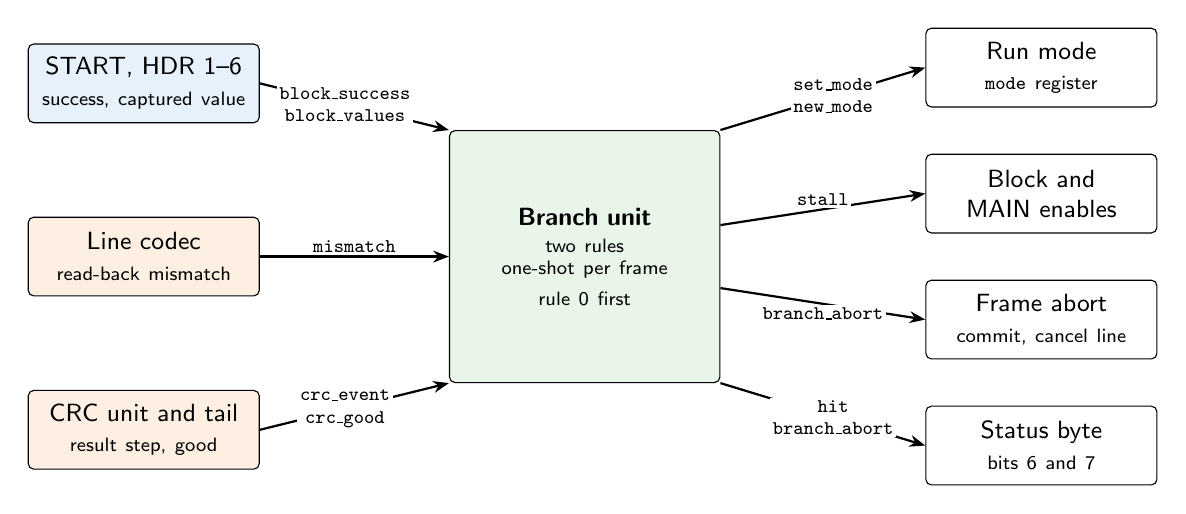
\begin{tikzpicture}[
  box/.style={draw,rounded corners=2pt,align=center,font=\small\sffamily,minimum height=1cm,text width=2.7cm},
  arr/.style={-{Stealth[length=2mm]},thick},
  lab/.style={font=\scriptsize\ttfamily,align=center,fill=white,inner sep=1pt}]
\node[box,fill=rxc] (blk) at (0,2.2) {START, HDR 1--6\\\scriptsize success, captured value};
\node[box,fill=txc] (codec) at (0,0) {Line codec\\\scriptsize read-back mismatch};
\node[box,fill=txc] (crc) at (0,-2.2) {CRC unit and tail\\\scriptsize result step, good};
\node[box,fill=outc,minimum height=3.2cm,text width=3.2cm] (bu) at (5.6,0) {\textbf{Branch unit}\\[2pt]\scriptsize two rules\\one-shot per frame\\rule 0 first};
\node[box] (mode) at (11.4,2.4) {Run mode\\\scriptsize \sig{mode} register};
\node[box] (en) at (11.4,0.8) {Block and MAIN enables};
\node[box] (ab) at (11.4,-0.8) {Frame abort\\\scriptsize commit, cancel line};
\node[box] (st) at (11.4,-2.4) {Status byte\\\scriptsize bits 6 and 7};
\draw[arr] (blk.east) -- node[lab,pos=0.45]{block\_success\\block\_values} (bu.north west);
\draw[arr] (codec) -- node[lab,above]{mismatch} (bu);
\draw[arr] (crc.east) -- node[lab,pos=0.45]{crc\_event\\crc\_good} (bu.south west);
\draw[arr] (bu.north east) -- node[lab,pos=0.55]{set\_mode\\new\_mode} (mode.west);
\draw[arr] (bu.east) ++(0,0.4) -- node[lab,above]{stall} (en.west);
\draw[arr] (bu.east) ++(0,-0.4) -- node[lab,below]{branch\_abort} (ab.west);
\draw[arr] (bu.south east) -- node[lab,pos=0.55]{hit\\branch\_abort} (st.west);
\end{tikzpicture}
\end{center}

A sixth output, \sig{line\_watch}, is not an action at all: it tells the chain to keep a write frame open until its last bit has left the pin (Section~\ref{sec:watch}).

%=====================================================================
\section{Ports}

\begin{center}
\begin{tabularx}{\linewidth}{@{}l l L@{}}
\toprule
Port & Dir & Meaning \\
\midrule
\sig{cfg\_we}, \sig{cfg\_sel} & in & Configuration write; \sig{cfg\_sel} 8 is rule 0, 9 is rule 1 (\sig{BRANCH 0} and \sig{BRANCH 1}). \\
\sig{cfg\_rule/mask/value} & in & The three operand bytes of \sig{BRANCH}. \\
\sig{block\_success} & in & One bit per block, START to \sig{HDR 6}; high from the clock a block finishes until the frame ends. \\
\sig{block\_values} & in & The eight-bit value of each block: what a read block received (or compared), what a write block sent. \\
\sig{mismatch} & in & From the line codec: the pad did not read back the level the chip drove, at this bit's check point. \\
\sig{crc\_event}, \sig{crc\_good} & in & The tail is pushing the CRC result entry this clock, and whether the check passed. \\
\sig{in\_frame} & in & START has succeeded (\sig{block\_success[0]}); rules only look inside a frame. \\
\sig{frame\_reset} & in & The frame is ending (complete, abort, timeout, halt). \\
\midrule
\sig{stall} & out & Hold every block and MAIN this clock. \\
\sig{set\_mode}, \sig{new\_mode} & out & Change the run mode to read (1) or write (2). \\
\sig{hit} & out & A rule took its \sig{HIT} action (registered). \\
\sig{branch\_abort} & out & Abort the frame (registered). \\
\sig{line\_watch} & out & A read-back rule is set: hold write frames open until the line is idle. \\
\bottomrule
\end{tabularx}
\end{center}

%=====================================================================
\section{Configuration}

Each rule is five small registers, loaded from one \sig{BRANCH} instruction:

\begin{center}
\begin{bytefield}[bitwidth=3.9em]{8}
\bitheader[endianness=big]{0-7}\\
\begin{rightwordgroup}{\sig{cfg\_rule}}
\bitbox{2}{\sig{ruleHit}} & \bitbox{2}{\sig{ruleMiss}} & \bitbox{1}{\sig{ruleSrc}} & \bitbox{3}{\sig{ruleBlock}}
\end{rightwordgroup}\\
\begin{rightwordgroup}{\sig{cfg\_mask}}
\bitbox{8}{\sig{ruleMask}}
\end{rightwordgroup}\\
\begin{rightwordgroup}{\sig{cfg\_value}}
\bitbox{8}{\sig{ruleValue}}
\end{rightwordgroup}
\end{bytefield}
\end{center}

\begin{itemize}
\item \sig{ruleOn} is set when the first byte is not zero, so \sig{BRANCH n} with byte 1 = \texttt{00} turns a rule off. (A rule whose actions are both KEEP is still on; that is how \sig{line\_watch} is set without changing anything else.)
\item Writing a rule also clears its \sig{fired} flag, so a rule rewritten mid-frame can act again in that frame.
\item The actions are \texttt{00} KEEP, \texttt{01} READ, \texttt{10} WRITE and \texttt{11} ABORT, the same for \sig{HIT} and \sig{MISS}.
\end{itemize}

%=====================================================================
\section{How one rule decides}

Both rules are the same logic, written as a loop over \sig{r} = 0, 1. A rule has two kinds of source, picked by \sig{ruleSrc}.

\subsection{Source 0: a block's value}

\begin{lstlisting}
watched[r]   = block_values[ruleBlock[r]]
matched[r]   = ((watched[r] ^ ruleValue[r]) & ruleMask[r]) == 0
fireBlock[r] = ruleOn[r] && !ruleSrc[r] && !fired[r] && in_frame
               && ruleBlock[r] < 7 && block_success[ruleBlock[r]]
\end{lstlisting}

\sig{watched} is an eight-way multiplexer over the block values. The match is a masked compare: every bit set in \sig{MASK} must equal the same bit of \sig{VALUE}; bits outside the mask are ignored, so \sig{MASK} = \texttt{00} always matches and \sig{MASK} = \texttt{01} tests one bit. The rule \emph{fires} on the first clock its block shows success. \sig{BLOCK} = 7 never fires (there is no block 7; MAIN cannot be watched).

\subsection{Source 1: an event on the line}

\begin{lstlisting}
lineEvent[r] = (ruleBlock[r] == 0) ? mismatch
                                   : (ruleBlock[r] == 1) && crc_event
lineHit[r]   = (ruleBlock[r] == 0) || crc_good
fireLine[r]  = ruleOn[r] && ruleSrc[r] && !fired[r] && in_frame && lineEvent[r]
\end{lstlisting}

\begin{itemize}
\item \sig{BLOCK} = 0, read-back: fires on the first bit where the pad disagrees with what the chip drove. A mismatch always counts as a hit, so only \sig{HIT} is used. This is CAN arbitration: drive recessive, see dominant, you have lost.
\item \sig{BLOCK} = 1, CRC: fires when the tail emits the CRC result. \sig{HIT} if the CRC was good, \sig{MISS} if it was bad.
\item Any other \sig{BLOCK} with \sig{SRC} = 1 never fires.
\end{itemize}

\subsection{From a firing rule to an action}

\begin{lstlisting}
fire[r]    = fireBlock[r] || fireLine[r]
tookHit[r] = (fireLine[r] && lineHit[r]) || (fireBlock[r] && matched[r])
action[r]  = (fireLine[r] ? lineHit[r] : matched[r]) ? ruleHit[r] : ruleMiss[r]
\end{lstlisting}

\sig{tookHit} feeds the status bit; \sig{action} is what the rule asks for this clock. A rule that does not fire still has an \sig{action} value, but it is ignored.

%=====================================================================
\section{Two rules, one answer}

\begin{lstlisting}
chosen = KEEP
if      (fire[0] && action[0] != KEEP) chosen = action[0]
else if (fire[1] && action[1] != KEEP) chosen = action[1]
\end{lstlisting}

Rule 0 wins only if it actually asks for something. If rule 0 fires with KEEP and rule 1 fires with READ in the same clock, the frame switches to read. Both rules still count for the status: \sig{hit} is the OR of both \sig{tookHit} bits.

In practice the two rules rarely fire together. They usually watch different blocks (for example, rule 0 on the address, rule 1 on a command byte), or one watches a block and the other the line.

%=====================================================================
\section{One shot per frame}

Each rule has a \sig{fired} flag. It is set in the clock the rule fires and cleared by \sig{frame\_reset} (or by rewriting the rule). While it is set the rule cannot fire again. Two reasons:

\begin{itemize}
\item \sig{block\_success} stays high for the rest of the frame once a block has finished. Without the flag a block rule would fire on every clock after that.
\item A read-back rule should act on the first mismatch, not on every later bit of a frame it has already given up.
\end{itemize}

%=====================================================================
\section{Outputs and timing}\label{sec:timing}

Some outputs are combinational and act in the same clock the rule fires; others are registered and act one clock later. The split is deliberate.

\begin{center}
\begin{tabularx}{\linewidth}{@{}l >{\raggedright\arraybackslash}p{3.4cm} L@{}}
\toprule
Output & When & Why \\
\midrule
\sig{stall} & same clock, and the clock after an abort & \sig{|fireBlock || internal\_abort}. Freeze the chain while a block rule decides, so the next block cannot start in the old mode. \\
\sig{set\_mode}, \sig{new\_mode} & same clock & The chain loads \sig{mode} at the end of this clock, so the next block starts in the new mode. \\
\sig{branch\_abort} & one clock later (\sig{internal\_abort}) & Abort fans out to the frame buffer, the codec and the status; registering it keeps the path from the block values to all of them short. \\
\sig{hit} & one clock later (\sig{internal\_hit}) & Only feeds a status flag. \\
\bottomrule
\end{tabularx}
\end{center}

Both registered outputs are suppressed if \sig{frame\_reset} arrives in the same clock, so a rule firing at the very end of a frame cannot leak into the next one.

\begin{center}
\begin{tikztimingtable}[timing/slope=0.1,xscale=1.2,yscale=1.1]
\sig{clk}                 & 12{C} \\
\sig{block\_success[2]}   & 2L 10H \\
\sig{fireBlock[0]}        & 2L 2H 8L \\
\sig{stall}               & 2L 2H 8L \\
\sig{set\_mode}           & 2L 2H 8L \\
\sig{mode}                & 4D{read} 8D{write} \\
\sig{fired[0]}            & 4L 8H \\
\sig{HDR 3 enabled}       & 4L 8H \\
\end{tikztimingtable}
\captionof{figure}{A rule on \sig{HDR 2} that switches to write: it fires in the first clock \sig{HDR 2} shows success, the chain stalls for that clock, and \sig{HDR 3} starts in the next clock with the new mode already in place.}
\end{center}

\begin{center}
\begin{tikztimingtable}[timing/slope=0.1,xscale=1.2,yscale=1.1]
\sig{clk}                 & 12{C} \\
\sig{fire[r]}, ABORT      & 2L 2H 8L \\
\sig{internal\_abort}     & 4L 2H 6L \\
\sig{stall}               & 2L 4H 6L \\
\sig{frame abort}         & 4L 2H 6L \\
\sig{tx\_cancel}          & 6L 2H 4L \\
\end{tikztimingtable}
\captionof{figure}{An abort: the frame aborts one clock after the rule fires, the stall covers that clock too, and the line codec drops its queued bits one clock after that (\sig{tx\_cancel} is registered in the chain).}
\end{center}

A line rule (read-back or CRC) does not stall the chain: the bit is already on the wire and the chain cannot take it back. A read-back abort therefore stops the line about two clocks after the mismatch check, well inside the bit; with ASYNC timing the check is mid-bit, so the chip stops driving within the bit it lost.

\paragraph{The cost of the stall.} One system clock per block rule per frame. Every standard ProEm runs has at least two system clocks per bit, and the stall falls between blocks, so no bit is lost.

%=====================================================================
\section{What the chain does with it}

\begin{itemize}
\item \textbf{Mode.} \sig{mode} is loaded from \sig{RUN}'s mode when the chain is armed, from \sig{new\_mode} on \sig{set\_mode}, and back to the \sig{RUN} mode at every frame end. The mode decides which blocks run (\sig{GRP} = \texttt{01} only when reading, \texttt{10} only when writing) and which way a MAIN with \sig{DIR} = follow goes.
\item \textbf{Enables.} \sig{stall} is ANDed out of every header's enable and MAIN's enable.
\item \textbf{Abort.} \sig{branch\_abort} is one of the chain's abort sources, but a gentler one. It \emph{commits} what has been captured so far instead of rolling it back, so the host sees the value that caused the abort (an SWD acknowledge, say). It also cancels whatever the line codec still has queued (\sig{cancel\_now}), and the frame ends with its status entry as usual.
\item \textbf{Status.} Bit 6 of the frame's status byte is set if any rule took its \sig{HIT} action during the frame (\sig{hit\_seen}); bit 7 if a branch aborted it. An abort on \sig{HIT} therefore reports \texttt{0xC2}, on \sig{MISS} \texttt{0x82}.
\end{itemize}

\subsection{\sig{line\_watch}}\label{sec:watch}

\sig{line\_watch} is high while either rule is on with \sig{SRC} = 1 and \sig{BLOCK} = 0. A write frame normally completes as soon as MAIN has handed its last entry to the codec, a few bit times before that bit leaves the pin. A late mismatch would then arrive after the frame had ended and be lost. With \sig{line\_watch} the chain waits (\sig{finish\_wait}) until the codec reports the line free before completing, so the read-back rule sees every bit.

The same signal is useful on its own. A rule \texttt{F0 08 00 00} (both actions KEEP, read-back) changes nothing but keeps write frames open until the line is idle. The K-Line and SDI-12 tests use it so that the next frame is not armed while the last stop bit is still being sent.

%=====================================================================
\section{Worked examples}

\subsection{I\textsuperscript{2}C target: direction from the R/W bit}

\sig{HDR 2} captures the R/W bit with \sig{ANY}. Rule \texttt{F0 92 01 01}: \sig{HIT} = WRITE, \sig{MISS} = READ, \sig{SRC} = 0, \sig{BLOCK} = 2, \sig{MASK} = \texttt{01}, \sig{VALUE} = \texttt{01}. If the controller asked to read (R/W = 1), the chip switches to write and MAIN (\sig{DIR} = follow) sends the loaded \sig{DATA}; otherwise it reads the controller's bytes. The status is \texttt{41} for a read (bit 6: the rule hit) and \texttt{01} for a write.

\subsection{SWD-style acknowledge}

\sig{HDR 2} reads the three-bit acknowledge. Rule \sig{HIT} = READ, \sig{MISS} = ABORT, \sig{BLOCK} = 2, \sig{MASK} = \texttt{07}, \sig{VALUE} = \texttt{01}. OK continues into the data phase; WAIT or FAULT aborts with \texttt{0x82}, and the host has already received the acknowledge value because a branch abort commits what was captured.

\subsection{CAN-style arbitration}

The chip drives an open-drain line and reads it back. Rule \sig{HIT} = ABORT, \sig{SRC} = 1, \sig{BLOCK} = 0. On the first bit where the chip sends recessive but reads dominant, the frame aborts with \texttt{0xC2} and the chip stops driving within that bit; the winning node's frame continues untouched.

\subsection{Acting on the CRC}

Rule \sig{SRC} = 1, \sig{BLOCK} = 1 fires when the tail emits the CRC result: \sig{HIT} if the check passed, \sig{MISS} if not. With \sig{MISS} = ABORT a bad frame is reported as aborted (\texttt{0x82}) instead of complete.

%=====================================================================
\section{Verification}

\begin{center}
\begin{tabularx}{\linewidth}{@{}l L@{}}
\toprule
Check & What it covers \\
\midrule
\sig{formal/branch\_unit.sby} & Unbounded proof against a model of the \sig{BRANCH} rules: masked compare, hit and miss actions, read-back and CRC sources, rule 0 before rule 1, each rule acting at most once per frame, and the timing of \sig{stall}, \sig{hit}, \sig{branch\_abort} and \sig{line\_watch}. \\
\sig{t\_branch} & SWD-style acknowledge (OK continues, WAIT and FAULT abort); CAN-style arbitration won and lost. \\
\sig{t\_i2c\_target} & Direction from the R/W bit, with repeated START. \\
\sig{t\_modes} & Rule 1 on its own value, rule 0 on another, in the same program. \\
\sig{t\_random\_branch} & 600 random programs: a rule on a captured header with random mask, value, actions and starting mode, then a read-only and a write-only header; checks which header runs, the data returned and the status byte. \\
\sig{t\_standards} & Read-back rules used only for \sig{line\_watch} (K-Line, SDI-12). \\
\bottomrule
\end{tabularx}
\end{center}

The one combination without a pin-level test is a rule on the CRC result (\sig{SRC} = 1, \sig{BLOCK} = 1). The formal proof covers it inside the module, and the CRC tests cover the \sig{crc\_event} and \sig{crc\_good} it relies on, but no test yet runs the two together through the whole chip.

%=====================================================================
\section{Signal glossary}

\begin{center}
\begin{tabularx}{\linewidth}{@{}l L@{}}
\toprule
Signal & Meaning \\
\midrule
\sig{ruleHit}, \sig{ruleMiss} & Action on a match and on a miss. \\
\sig{ruleSrc}, \sig{ruleBlock} & What the rule watches: a block (0) or a line event (1), and which one. \\
\sig{ruleMask}, \sig{ruleValue} & The masked compare for block rules. \\
\sig{ruleOn} & The rule is configured (byte 1 not zero). \\
\sig{watched} & The value of the block the rule watches. \\
\sig{matched} & The watched value passes the masked compare. \\
\sig{fireBlock}, \sig{fireLine} & The rule acts this clock, from a block or from the line. \\
\sig{lineEvent}, \sig{lineHit} & The line event happened, and whether it counts as a hit. \\
\sig{fire}, \sig{action}, \sig{tookHit} & Per rule: acting, what it asks for, and whether it took \sig{HIT}. \\
\sig{chosen} & The action that wins this clock (rule 0 first, KEEP does not win). \\
\sig{fired} & The rule has acted in this frame. \\
\sig{internal\_hit}, \sig{internal\_abort} & Registered \sig{hit} and \sig{branch\_abort}. \\
\bottomrule
\end{tabularx}
\end{center}

\end{document}
